\chapter{Foundations}
\label{sec:foundations}

\section{ROS – Robot Operating System}
\label{sec:ros}

Das Robot Operating System (ROS) ist ein Open Source Programmiergerüst (Framework)  zur Programmierung von Software für Roboter. ROS bietet zahlreiche Bibliotheken und Tools zum organisieren von komplexen und unterschiedlichen Aufgaben, um ein robustes Zugsamenspiel zwischen den verschiedenen Hardwarekomponenten einer oder mehrerer Roboterplattformen zu gewährleisten.  Im wesentlichen besteht ROS aus Treiber, die Daten von Sensoren wie Kameras, Laserscannern und GPS-Modulen auslesen, Algorithmen zum erstellen von Karten, Pfadplanung oder allgemeiner Navigation, der Infrastruktur, welche die Komponenten des Robotersystems miteinander verbindet und die Datenpakete zwischen den Prozessen verwaltet und Werkzeuge, zur Visualisierung des Roboters, der Aufnahme von Sensordaten und zur Fehleranalyse. 
Ein ROS-System besteht aus einzelnen Programmen, die in ROS nodes (Knoten) genannt werden. Die Programme kommunizieren untereinander über sogenannte edges (Kanten), welche die Datenströme darstellen. Ein Konten kann Datenströme senden, dann published er eine Topic, sodass ein anderer Knoten auf diese Topic subscriben, also diese Nachricht empfangen kann. Die Knoten und Kanten werden über einen Master überwacht, den roscore. 
Anleitungen für die Installation und Herangehensweise sind unter wiki.ros.org zu finden. Fragen werden durch die große Online-Community von Nutzern und Entwicklern beantwortet. 
Auf Internetseiten wie github.com werden auf Grundlage der ROS-Bibliothek vorprogrammierte oder fertige Programme geteilt, wodurch Programmieraufwand für neue Projekte reduziert werden kann, da oft auf diese bereits bestehende Programme aufgebaut, oder diese komplett übernommen werden. Daraus lässt sich der größte Vorteil von ROS ableiten, das Zeitersparnis.
ROS kann in jeder modernen Programmiersprache implementiert werden, jedoch wird es aktuell primär in Python, C++ und Lisp implementiert. Als Betriebssystem wird ein Unix-basiertes Betriebssystem vorausgesetzt. 
Im Fachbereich Verteilte Systeme der Universität Kassel existieren bereits viele ROS Applikationen. Da diese Arbeit in das bestehende ROS-System integriert werden soll, wird mit dieser Arbeit eine ROS-Applikation entwickelt. Entsprechend wurde das Betriebssystem Ubuntu 18.04 und die Programmiersprache C++ als Grundlage verwendet. 





\section{ConceptNet}
\label{sec:cn}

Conceptnet ist ein multilinguales semantisches Netzwerk, welches menschliches Allgemeinwissen in eine für Computer verständliche Sprache übersetzen soll. Netzwerke sind Datensätze,welche aus Begriffen (Knoten) und derer Beziehungen (Kanten) bestehen\cite{sowa1987semantic}. Bei semantischen Netzwerken bestehen die Kanten aus Wörtern, die eine Bedeutung der Beziehung zwischen zwei Knoten zuordnen. Semantische Netzwerke dienen in der Computerlinguistik als objektorientierte Wissensrepräsentationsmethode (WRM) und sind dem Bereich der künstlichen Intelligenz zuzuordnen\cite{helbig2013semantische}. 
Oft werden Netzwerke als Graphen dargestellt. 

\begin{figure}[h]

	\begin{center}
	
	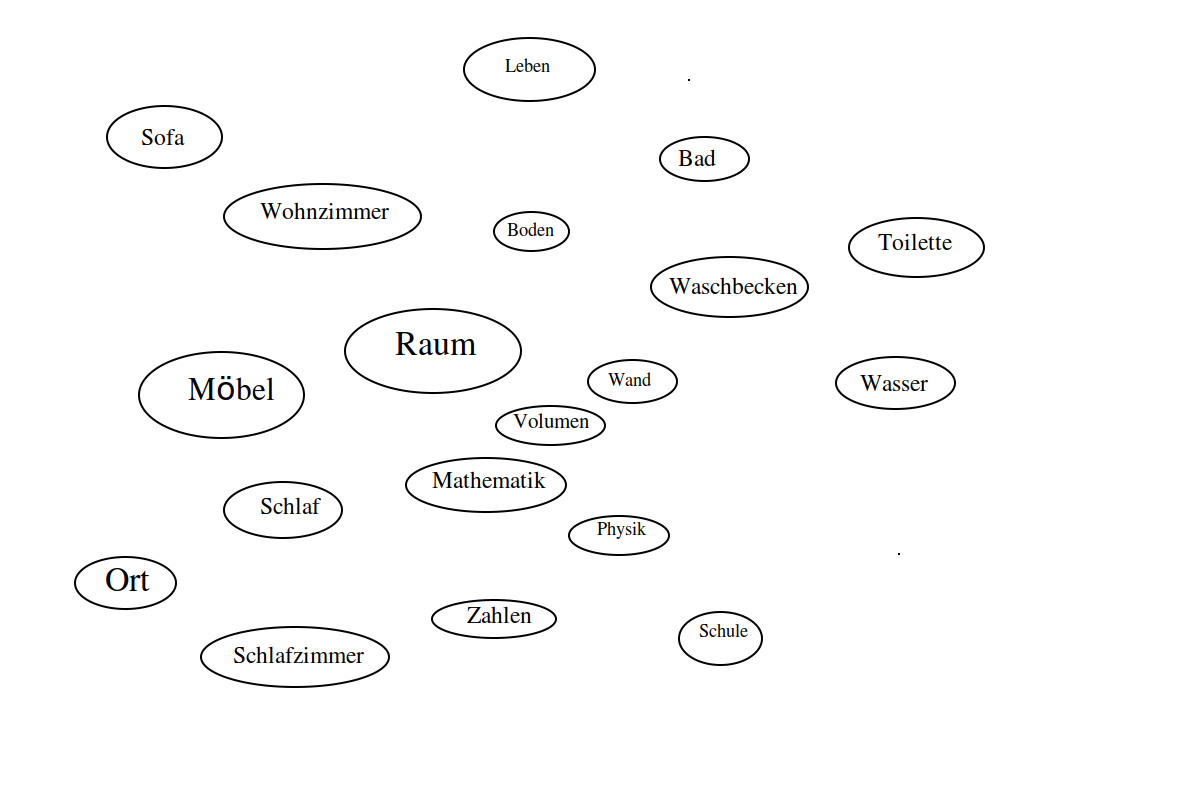
\includegraphics[width=18cm]{images/Netzwerk.png}
	
	\caption{Netzwerk}
	
	\label{netzwerk_Bild}
	
	\end{center}
	
	
\end{figure}

In Abbildung … ist ein semantisches Netzwerk dargestellt. Zu sehen ist, wie die Begriffe, zum Beispiel Wohnzimmer und Raum, zueinander in Beziehung stehen. Ein Wohnzimmer ist ein (IsA) Raum. IsA ist eine der 36 in Conceptnet Version 5.5 definierten Kernbeziehungen, die eine Deutung der Beziehung ermöglichen. Conceptnet Version 3 hat 26 Kernbeziehungen\cite{havasi2007conceptnet}. Weitere Beziehungen sind RelatedTo, welche einen Zusammenhang zweier Begriffe beschreibt, diese aber nicht genauer benennen kann und AtLocation, diese lässt auf einen Standort schließen. Ein Raum ist ein Ort, an dem sich Möbel befinden. 
In Conceptnet werden die Beziehungen in zwei Klassen eingeteilt, in symmetrische und asymmetrische Beziehungen. Zu den symmetrischen Beziehungen gehören beispielsweise RelatedTo, Synonym und Antonym. Hierbei handelt es sich um generellere Beziehungen, hingegen sind asymmetrische Beziehungen wie AtLocation, IsA, PartOf und UsedFor genauer definiert in Bezug auf ihre Deutungen. Eine weitere Eigenschaft des semantischen Netzwerkes ist das Kantengewicht, welches die Wichtigkeit der Beziehung abbildet. Ein Bett wird in Conceptnet mit einer Gewichtung von 10,9 in Beziehung zu Möbel gesetzt, eine Toilette mit einer Gewichtung von 0,17. Daraus lässt sich weiterer Kontext erschließen. 

\begin{figure}[h]
	
	\begin{center}
		
		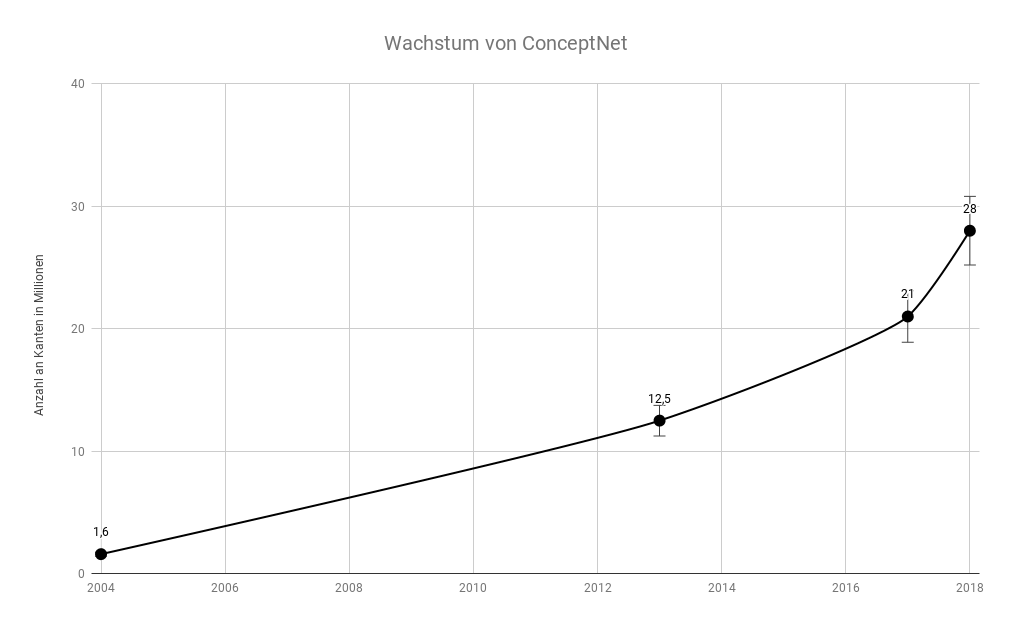
\includegraphics[width=16cm]{images/Wachstum_von_ConceptNet.png}
		
		\caption{Wachstum von Conceptnet}
		
		\label{wachstum_cn}
		
	\end{center}
	
	
\end{figure}


Abbildung ... zeigt das Wachstum von Conceptnet in Abhängigkeit der Anzahl der Beziehungen im zeitlichen Verlauf. Die Version 5.5 von Conceptnet weißt über 21 Millionen solcher Beziehungen auf und umfasst ach Millionen Begriffe. Da Conceptnet stetig weiterentwickelt wird, auf neue Ressourcen zugreift, vergrößert sich das Netzwerk und erzielt bessere Resultate. Bei der Version 5.6 wird die Anzahl der Beziehungen auf über 28 Millionen geschätzt, im Jahr 2004 waren es nur knapp zwei Millionen. 
Das Wissen von Conceptnet basiert ursprünglich auf Crowdsourcing Datensätzen wie wiktionary, DBpedia und Open-Mind-Common-Sense, auf Spielen wie verbosity und ndaya.jp und Expertenwissen von Wordnet, OpenCyc und JMDict. Ein neuer Ansatz ist Wissen von Word Embeddings, wie word2vec und GloVe, mit in Conceptnet zu integrieren. In \cite{speer2017conceptnet} werden unter dem Synonym ConceptNet Numberbatch bereits erste Erfolge nachgewiesen.

Zehn verschiedene Sprachen bilden den Kern von Conceptnet, in Summe sind über 300 Sprachen vertreten. Conceptnet hat sich in der Vergangenheit gegen andere semantische Netzwerke behauptet. Lediglich der Vergleich zu Cyc ist nicht genau zu validieren, da diese Plattform seit 2015 nicht mehr öffentlich zugänglich ist. Conceptnet hingegen ist ein Open Source Netzwerk und bietet die Möglichkeit über eine Web-API in eigene Anwendungen integriert zu werden. Wissenspakete im Json-Format können angefragt und für spezielle Aufgaben weiterverarbeitet werden. 
Die große Menge an Begriffen und der Wissensgehalt durch die Beziehungen von Conceptnet sind eine gute Voraussetzung als Wissensbasis für Künstliche Intelligenz und bieten eine Grundlage für diese Arbeit. 
\cite{liu2004conceptnet}
\cite{havasi2007conceptnet}
\cite{speer2013conceptnet}
\cite{speer2017conceptnet} 

\begin{align}
E &= mc^2
\end{align}





